\documentclass[11pt]{article}
% \usepackage{xcolor}
% \usepackage{glossaries}
% \usepackage{lingmacros}
% \usepackage{tree-dvips}
\usepackage[utf8]{inputenc}
\usepackage{fancyhdr}
% \usepackage{xr}
\usepackage{graphicx}
\usepackage{wrapfig,lipsum}
\usepackage[tocflat]{tocstyle}
% \usepackage[bottom]{footmisc}
\usepackage[ngerman, num]{isodate}
% \usepackage{fourier}
% \usepackage[parfill]{parskip}
\usepackage{hyperref}
% % * Set page layout
% % Seitenränder
\usepackage[a4paper,left=2.5cm,right=2.5cm,top=2cm,bottom=2cm]{geometry}
\usepackage{csvsimple}
% % * Set font 'Fira Sans Regular'
% \usepackage[sfdefault]{FiraSans}
% \usepackage[T1]{fontenc}
% \renewcommand*\oldstylenums[1]{{\firaoldstyle #1}}
\usepackage{enumerate}
\usepackage{tocloft}
\renewcommand{\cftsecleader}{\cftdotfill{\cftdotsep}}

%subsubsubsections
\usepackage{titlesec}

\setcounter{secnumdepth}{4}
\setcounter{tocdepth}{4}

\titleformat{\paragraph}
{\normalfont\normalsize\bfseries}{\theparagraph}{1em}{}
\titlespacing*{\paragraph}
{0pt}{3.25ex plus 1ex minus .2ex}{1.5ex plus .2ex}

\newcommand{\subsubsubsection}[1]{\paragraph{#1}}



% Kopfzeile
\linespread{1.25}
\usepackage{fancyhdr}
\pagestyle{fancy}


\renewcommand{\refname}{}

% Bilder Referenzen
\usepackage{graphicx}
\graphicspath{ {./bilder/} }

\renewcommand{\listfigurename}{}
\makeatother
\renewcommand{\figurename}{Abbildung}
%\renewcommand{\thefigure}{\thefigure \arabic{figure}}
\renewcommand{\cftfigfont}{Abb. }




\renewcommand{\contentsname}{Inhalt}


\usepackage{booktabs}% http://ctan.org/pkg/booktabs
\newcommand{\tabitem}{~~\llap{\textbullet}~~}

\usepackage{makecell}
\usepackage{longtable}

\newcommand*{\source}[3]{%
  \caption[#1 \newline #2 \newline #3]{#1}
}

\usepackage{xltabular}

\begin{document}
    \begin{titlepage}
    \begin{center}
        
\includegraphics[width=0.2\textwidth]{Logo_BSZ_ET.png}\\
        \vspace*{1cm}
        {\huge{Zwischensysteme}}
 
        \vspace{0.5cm}
         
        \vspace{1.5cm}
 
        \textbf{Christian Schülke\\Elias Martin\\Lena Höhn\\Laura Pech}\\
        Auszubildende Fachinformatiker für Anwendungsentwicklung und Systemintegration\\

        \vfill
 



        \vfill
        {\huge\textbf{Projektarbeit}}
        
    
        \vspace{1cm}
        {\Huge 2019 / 2020}\\
        \vspace{0.8cm}
        IF 18 - 4\\
        S5\\
        Betreut von Herr Räntzsch\\
        BSZ für Elektrotechnik\\
        Strehlener Pl. 2, 01219 Dresden\\
        \today
             
    \end{center}
 \end{titlepage}
    \pagebreak
    \tableofcontents
    \pagebreak
    \section{Vorbereitung}
    \subsection{Begriffserklärung Zwischensystem und Endsystem}

    Ein \textbf{Endsystem} oder Endgerät ist ein Computer oder ein anderes Peripheriegerät, an welchem keine weiteren Geräte angeschlossen sind. \\
    Beispiele für Endsysteme sind:
    \begin{itemize}
        \item Drucker
        \item Geldautomat
        \item Surfstation
        \item Lautsprecher
        \item Kamera
    \end{itemize}
    \vspace{0cm}
    Außerdem muss es \textbf{Zwischensysteme} geben, die gesendete Datenpakete an die richtige Adresse weiterleiten. \\
    Solche Zwischensysteme sind Switches, Bridges und Router. 


\subsection{Nutzen der Protokollschichten des Osi-Modells}

    Das OSI Modell ist ein Modell, welches die Ebenen die ein Netzwerk ausmachen beschreibt.

    \renewcommand{\tabcolsep}{1pt}
\begin{longtable}{@{}p{0.3\textwidth}@{\hspace{3em}}p{0.6\textwidth}}
    \\\hline
    \makecell[l]{Bitübertragungsschicht \\ (Physical Layer)}
        & 
        \begin{itemize}
            \item elektrische / physische Übertragung der Daten 
        \end{itemize}
        
    \\\hline

    \makecell[l]{Sicherungsschicht \\ (Data Link Layer)}
        &
        \begin{itemize}
            \item alle Vorkehrungen, die dafür sorgen, dass aus der physikalischen Übertragung ein verlässlicher Datenfluss wird
        
        \end{itemize}
    \\\hline
    
    \makecell[l]{Vermittlungsschicht \\ (Network Layer)}
        &
        \begin{itemize}
            \item Komponenten und Protokolle, die an der Verbindung zwischen Rechnern beteiligt sind - das sogenannte Routing - Weiterleiten von Daten in andere logische und oder physikalisch inkompatible Netzwerke
        \end{itemize}
    \\\hline
    
    \makecell[l]{Transportschicht \\ (Transport Layer)}
        &
        \begin{itemize}
            \item verbindungsorientierte Protokolle wie TCP und verbindungslose Protokolle wie UDP
            \item ein wichtiger Aspekt dieser Schicht ist Multiplexing - Anbindung der Datenpakete an konkrete Prozesse auf den kommunizierenden Rechnern 
            \item Segmentierung des Datenstroms und Datenstauvermeidung
        \end{itemize}
    \\\hline

    \makecell[l]{Kommunikationssteuerungsschicht \\ (Session Layer)}
        &
        \begin{itemize}
            \item sichert Kommunikation zwischen kooperierenden Anwendungen oder Prozessen auf verschiedenen Rechnern
            \item organisiert und synchronisiert Datenaustausch
        \end{itemize}
    \\\hline

    \makecell[l]{Darstellungsschicht \\ (Presentation Layer)}
        &
        \begin{itemize}
            \item Konvertierung und Übertragung von Datenformaten, Datensätzen, Zeichensätzen, grafische Anweisungen und Dateidienste
            \item systemabhängige Darstellung von Daten
            \item Datenkompression, Verschlüsselung
            \item stellt sicher, dass Daten die von der Anwendungsschicht des einen Systems gesendet werden von der Anwendungsschicht eines anderen Systems gelesen werden können
        \end{itemize}
    \\\hline

    \makecell[l]{Anwendungsschicht \\ (Application Layer)}
        &
        \begin{itemize}
            \item unmittelbare Kommunikation zwischen Benutzeroberflächen der Anwendungsprogramme
            \item Das Anwendungsprogramm selbst zählt nicht dazu
        \end{itemize}
    \\\hline

    
\end{longtable}


    \begin{figure}[ht]
        \centering
        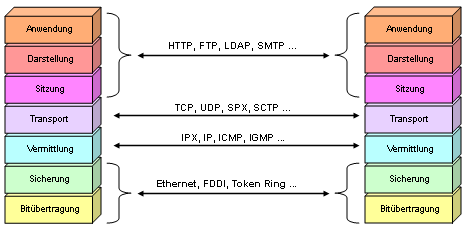
\includegraphics[width=\textwidth]{vorbereitung/Osi.png}
        \source{Osi Modell}{https://www.der-wirtschaftsingenieur.de/bilder/it/OSI-Modell3.PNG}{3.1.2020 14:30}
    \end{figure}
    \vspace{0cm}
    \textbf{Repeater}
    \\
    Ein Repeater verstärkt ganz simpel die elektronischen Signale und nutzt deswegen nur die 1. Schicht des OSI-Models. Der in der Abbildung unterhalb veranschaulichte HUB (Multi-Port-Repeater) sendet ein von PC0 gesendetes Paket an alle anderen PC’s weiter, da er keine Möglichkeit hat, an ein bestimmtes Gerät zu senden, da er keine MAC-Adressen speichert. Er teilt keine Broadcastdomäne.\\

    \begin{figure}[ht]
        \centering
        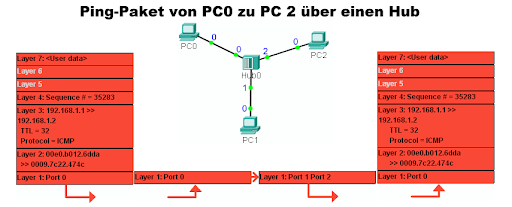
\includegraphics[width=\textwidth]{vorbereitung/ping_hub.png}
        \source{Ping über einen Hub}{https://www.tinohempel.de/info/info/netze/osi.htm}{8.1.2020 13:00}
    \end{figure}
    \vspace{0cm}
    \textbf{Bridge}
    \\
    Eine Bridge verbindet mehrere über Kabel verbundene Netzwerke / PCs miteinander, sodass sie ein einzelnes Netz repräsentieren. In Bezug auf das OSI Modell werden über die erste Schicht Signale versandt und über die zweite Schicht werden die Signale einem Zielort via einer Link-Layer-Address zugeordnet. In der folgenden Abbildung sieht man einen Switch (Multi-Port-Bridge), welcher die von PC0 gesendeten Pakete anhand der MAC-Adresse, aus dem entsprechenden Port, an PC2 weiterleitet. \\

    \begin{figure}[ht]
        \centering
        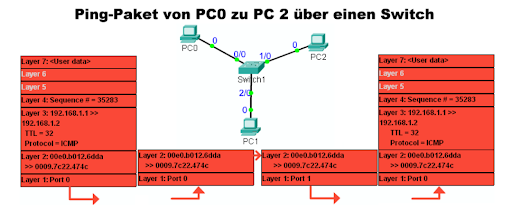
\includegraphics[width=\textwidth]{vorbereitung/ping_bridge.png}
        \source{Ping über einen Switch}{https://www.tinohempel.de/info/info/netze/osi.htm}{8.1.2020 13:00}
    \end{figure}
    \vspace{0cm}
    \textbf{Router}
    \\
    Ein Router verbindet mehrere Netzwerke miteinander. Anhand von Routing-Tabellen (statisch oder dynamisch) leitet er die Datenpakete in die entsprechende Netze oder über ein Default-Gateway weiter. Die Routing-Entscheidungen geschehen aufgrund von IP-Adressen (OSI-Layer 3) und ggf. weiteren Parametern z.B. anhand der Pfadkosten beim OSPF-Protokoll. PC0 sendet das Datenpaket an Router1 mit seiner IP-Adresse als Quelladresse und der Zieladresse (PC2). Der Router kennt das Zielnetz, da es direkt angeschlossen ist und sendet es an PC2 weiter.\\

    \begin{figure}[ht]
        \centering
        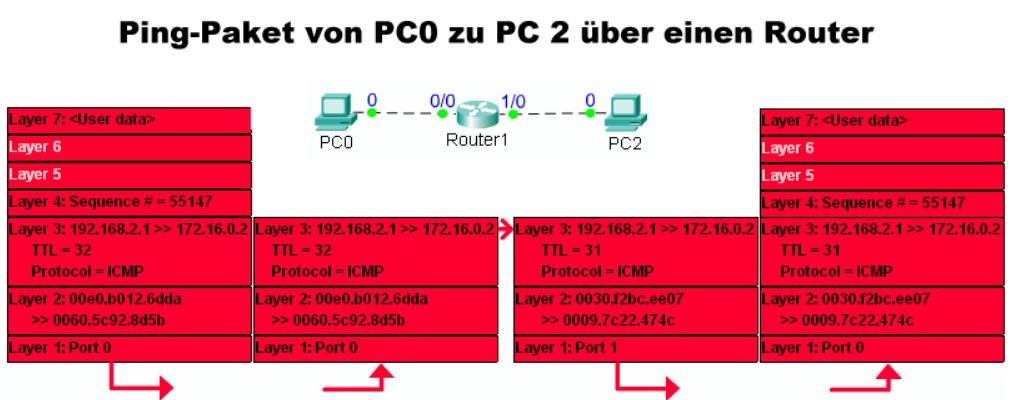
\includegraphics[width=\textwidth]{vorbereitung/ping_router.png}
        \source{Ping über einen Router}{https://www.tinohempel.de/info/info/netze/osi.htm}{8.1.2020 13:00}
    \end{figure}
    \vspace{0cm}
    \textbf{Gateway}
    \\
    Ein Gateway ist ein computer-ähnliches Gerät, welches eine Kommunikation zwischen zwei oder mehr unterschiedlichen Systemen herstellt. Ein Gateway kann Software oder Hardware sein. Um mit verschiedenen Arten von Netzwerken zu kommunizieren, muss der Netzwerk Gateway auf mehreren Schichten des OSI Modells operieren, unter Umständen auch auf allen 7, da er zum Beispiel Sessions erstellen und verwalten muss, Daten entschlüsseln und unterschiedliche physikalische und logische Adressen übersetzen muss. Wegen der vielen Aufgaben die ein Gateway gleichzeitig erledigen muss ist er um einiges langsamer, als die anderen oben genannten Geräte. Der Gateway, der in der Aufgabenstellung dargestellt wird greift auf alle 7 Layer zu und muss deswegen eine Software auf einem Computer sein, auf die ein Benutzer via einer Oberfläche zugreifen kann.\\

\subsection{Einordnung von Switch und Layer-3-Switch in Abbildung}

    \textbf{Switch}
    \\
    Ein Layer-2-Switch arbeitet mit Data-Link Layer-Adressen (MAC). Er benutzt also nur die Bitübertragungsschicht und die Sicherungsschicht. Er sendet die Daten weiter an einen fest angegebenen Punkt anhand der MAC-Adressen. \\
    Er ist als Äquivalent zur Bridge zu sehen. Denn er ist im Prinzip eine Multi-Port-Bridge und im Gegensatz zum HUB, erzeugt er keinen unnötigen Traffic, da nur an ein bestimmtes Ziel und nicht an alle gesendet wird (durch MAC-Adressen-Tabelle).\\
    \\
    \textbf{Layer-3-Switch}
    \\
    Ein Layer-3-Switch ist ein Switch, welcher um die Routing-Funktionen erweitert wurde und sonst alle Funktionen von einem Layer-2-Switch beibehält. Deshalb ist er mit dem Router aus Abbildung 1 gleichzusetzen. Durch die Erweiterung auf Layer 3 unterstützen diese Switches auch Inter-VLAN-Routings. Erweiterte Funktionen, wie NAT, IPSec oder Firewall-Filtering werden allerdings nicht unterstützt.



\subsection{Zweck und Header-Aufbau von ICMP, Nutzung des Protokolls in der Konsole unterschiedlicher Betriebssysteme}
    Das ICMP (Internet Control Message Protocol) tauscht Informations- und Fehlermeldungen über IPv4 in Rechnernetzen aus. Das Äquivalent in IPv6 heißt ICMPv6.\\
    Für jeden Rechner und Router ist es Standard, dass sie ICMP verstehen.\\
    ICMP Pakete dienen dazu Diagnose Informationen zurück an die Quelle zu senden, wenn der Router Pakete verwirft. Beispielsweise, wenn das Ziel nicht erreichbar ist oder die TTL abgelaufen ist.\\
    So wird zum Beispiel mit dem Befehl “ping” ein Test Datenpaket über das ICMP Protokoll gesendet.\\
    \begin{itemize}
        \item Zweck, Headeraufbau
        \item Nutzung in der Konsole unterschiedlicher Betriebssysteme
    \end{itemize}

    Der Befehl ping ist unter den meisten Betriebssystemen wie Windows, Linux (und anderen Unixartigen), Unix oder macOS, aber auch als Analysetool auf Geräten wie Routern nutzbar. Die Ausführung des Befehls und somit die Aussendung der ICMP Pakete unterscheiden sich jedoch je nach Betriebssystem, so sendet Windows eine begrenzte Anzahl an Paketen während Linux eine unbegrenzte Anzahl sendet und nur manuell abgebrochen werden kann.\\

    \begin{figure}[ht]
        \centering
        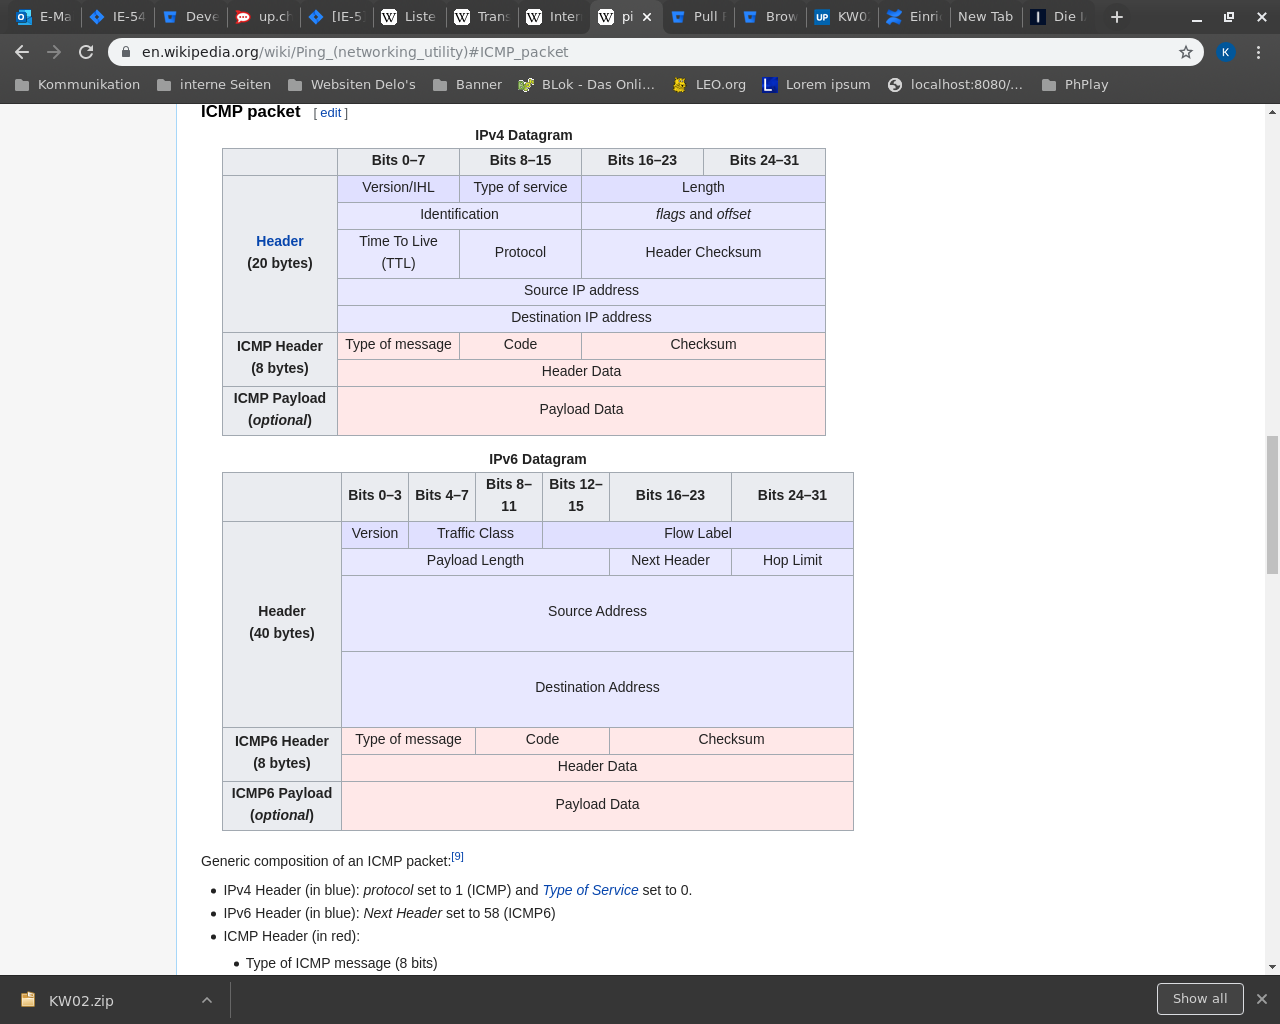
\includegraphics[width=0.5\textwidth]{vorbereitung/IPv4_IPv6_Datagramm.png}
        \source{IMCP Aufbau}{https://en.wikipedia.org/wiki/Ping\_\(networking\_utility\)\#ICMP\_packet}{2.1.2020 15:00}
    \end{figure}




\subsection{Peer-2-Peer Netzwerk entsprechend DFÜ-Modell}

    DDE bezeichnet die Datenendeinrichtung und stellt den Sender oder den Empfänger dar. Sie kontrolliert und steuert die Datenfernübertragung.\\
    DÜE bezeichnet die Datenübertragungseinrichtung. Sie ist die Verbindung zwischen den DDE’s und dem Netzwerk und wandelt die Daten in eine geeignete Form für die Übertragung um.\\
    Zwischen DDE und DÜE befindet sich eine serielle Schnittstelle (V.24, RS232), ein USB Kabel oder eine Funkverbindung wie Bluetooth.\\

    \begin{figure}[ht]
        \centering
        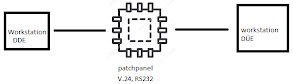
\includegraphics[width=0.5\textwidth]{vorbereitung/DFUE.png}
        \source{DFÜ Modell}{eigene Zusammenstellung}{}
    \end{figure}
\subsection{Skizze des Protokollstapels}

    \begin{figure}[ht]
        \centering
        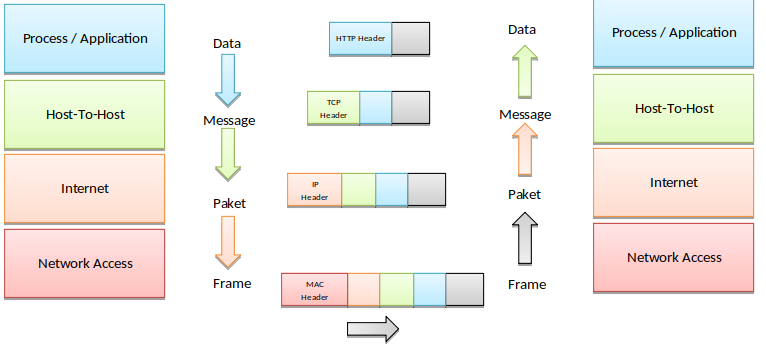
\includegraphics[width=0.5\textwidth]{vorbereitung/Protokollstapel.png}
        \source{Skizze eines Protokollstapels eines HTTP Requests}{eigene Zusammenstellung}{}
    \end{figure}

\subsection{Headerstruktur für HTTP, TCP, IPv4, IPv6 und Ethernet}

    \textbf{Http Response Header}
    \\
    Übergeben zusätzliche Informationen über die Antwort, die nicht in die Status Line passen. Sie Enthalten Informationen über den Server und weitere Zugänge zu der Quelle. Diese sind durch die Request-URI gekennzeichnet.\\

    \begin{figure}[ht]
        \centering
        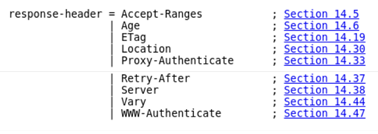
\includegraphics[width=0.5\textwidth]{vorbereitung/http_response_header.png}
        \source{HTTP Response Header}{http://www.coder-welten.de/glossar/request-und-response-18.html}{07.01.2020 15:00}
    \end{figure}

    \textbf{HTTP Request Header}
    \\
    Geben zusätzliche Informationen über den Request mit, wie über den Client selbst, zum Server. \\
    \begin{figure}[ht]
        \centering
        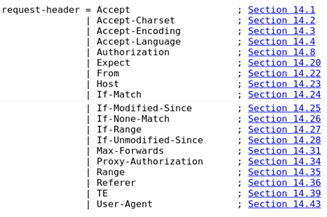
\includegraphics[width=0.5\textwidth]{vorbereitung/http_request_header.png}
        \source{HTTP Request Header}{http://www.coder-welten.de/glossar/request-und-response-18.html}{07.01.2020 15:00}
    \end{figure}

    \textbf{TCP Header}
    \\
    Dieser Header enthält die zur Kommunikation erforderlichen Daten und Dateiformat-beschreibende Informationen. Normalerweise sind TCP Header 20 Bytes lang, können aber mit den kaum genutzen Optionen erweitert werden.\\

    \begin{figure}[ht]
        \centering
        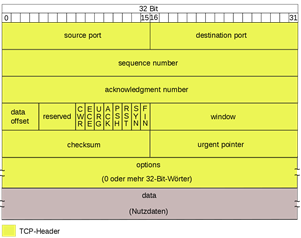
\includegraphics[width=0.5\textwidth]{vorbereitung/TCP_Header.png}
        \source{TCP Header}{https://upload.wikimedia.org/wikipedia/commons/thumb/f/fd/TCP\_Header.svg/1024px-TCP\_Header.svg.png}{2.1.2020 14:00}
    \end{figure}

    \textbf{IPv4 Header}
    \\
    Die Länge von IPv4 Header ist normalerweise 20 Bytes, kann aber mit bestimmten Optionen auf bis 60 Bytes erweitert werden.\\

    \begin{figure}[ht]
        \centering
        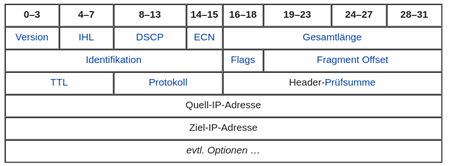
\includegraphics[width=0.5\textwidth]{vorbereitung/IPv4_Header.png}
        \source{IPv4 Header}{https://de.wikipedia.org/wiki/IPv4\#Header-Format}{2.1.2020 14:30}
    \end{figure}

    \textbf{IPv6 Header}
    \\
    Hat eine feste Länge von 40 Bytes. Optionale selten genutzte Daten können in Extension Headern zwischen Header und Payload gesendet werden.\\

    \begin{figure}[ht]
        \centering
        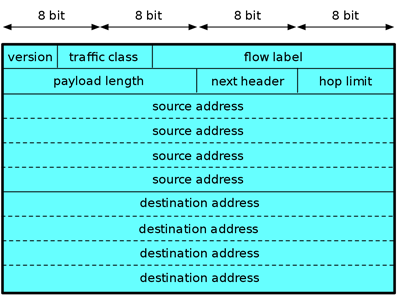
\includegraphics[width=0.5\textwidth]{vorbereitung/IPv6_Header.png}
        \source{IPv6 Header}{https://upload.wikimedia.org/wikipedia/commons/thumb/c/cd/IPv6\_Header.svg/1280px-IPv6\_Header.svg.png}{2.1.2020 14:45}
    \end{figure}

    \textbf{Ethernet}
    \\
    Enthält die Zieladresse (6 Bytes), Quell-MAC-Adresse (6 Bytes), das EtherType field (2 Bytes) und optional einen IEEE 802.1Q tag oder einen IEEE 802.1ad tag (4 Bytes).

\subsection{Analyse von Anweisungen für das Protokoll IPv6}
    \renewcommand{\tabcolsep}{1pt}
\begin{xltabular}{\textwidth}{@{}p{0.4\textwidth}@{\hspace{3em}}p{0.6\textwidth}@{}}
    \\\hline
    \makecell[l]{netsh interface ipv6 show interfaces \\ (füher ipv6 if)}
        &
    \makecell[l]{
        Pingt das angegebene Interface an und gibt dabei die link-layer-adress, die ipv6 Adressen die zu dem Interface gehören und das aktuelle MTU und die maximale Anzahl der MTU’s die das Interface unterstützen kann.\\
        Interface 1 ist ein Pseudo-Interface.\\
        zeigt an:\\
            \textbf{Index} - Bereichskennung \\
            \textbf{Met} - gibt die Pfadkosten an, je niedriger, desto besser, kann wenn es mehrere Routen gibt dazu verwendet werden zu entscheiden, welche Route verwendet wird\\
            \textbf{MTU} - maximale Anzahl an MTU’s die das Interface unterstützt\\
            \textbf{state} - status des Interfaces, ist Interface enabled Oder disabled\\
            \textbf{name} - Name des Interfaces
    }
    \\\hline
    ping -6 ::1
    &
    Pingt den localhost an. Das heißt es wird ein ICMP-Paket mit einem TTL Wert von 128 gesendet und kommt vom localhost wieder zurück.
    \\\hline
    ping -6 Adresse\%Bereichskennung
    &
    Pingt die Adresse über das in der Bereichskennung angegebene Interface an. Zum Beispiel wenn man die Adresse fe80::1\%SCHNITTSTELLE einen ping heraus sendet, wird ein ICMP Paket an die Link-Local-Adress fe80::1 über die Schnittstelle “SCHNITTSTELLE” an.
    \\\hline
    netsh interface ipv6 show route
    &
    \makecell[l]{
        Pingt jeden Hop bis zum Host an und verfolgt dabei die Route.\\
        Dabei werden ICMP-Pakete mit immer höher werdendem TTL-Wert ausgesandt, die dann nacheinander von den beteiligten Routern bearbeitet werden. Der höchste TTL-Wert entspricht dann dem des Hosts.\\
        Die Ausgabe zeigt dann die Hops bis zum Ziel an.\\
        Angezeigt werden:\\
            - Der wie vielte Hop wurde bewältigt\\
            - die Zeit die gebraucht wurde um den Hop zu bewältigen\\
            - die IP des Hops und die Benennung
    }

\end{xltabular}
    \pagebreak
    \section{Durchführung}
    \subsection{Versuchsaufbau}
\subsubsection{Installieren und Konfigurieren der Software auf den WS}
    \textbf{Planung}
    \begin{itemize}
        \item Zwei Win 8 Rechner starten
        \item Rechner per P2P verbinden
        \item Auf einer Maschine XAMPP installieren mit Auswahl nur Apache, auf der zweiten Maschine Wireshark installieren
        \item Auf beiden PC's Firewall deaktivieren
        \item DHCP auf statische IP’s umstellen: 10.0.0.2 \& 10.0.0.3
        \item Im xampp-Verzeichnis unter htdocs  die Seite hallo.htm einfügen
        \item Im browser die Seite über “localhost/hallo.htm” und “<IP>{\textbackslash}hallo.htm” aufrufen
    \end{itemize}
    \
    \underline{\textbf{DoD Schichtmodel}}\\
    \textbf{Network Access Schicht}\\
    (Die Schicht, auf der die Geräte physisch verbunden sind)
    \begin{itemize}
        \item Bei uns über internen virtuellen Switch gelöst
        \item MAC Adresse wird ausgelesen
    \end{itemize}
    \
    \textbf{Internet Schicht}
    \\
    (Die Schicht, die Netzwerkweite Verbindungen unabhängig von Übertragungsmedium ermöglicht)
    \begin{itemize}
        \item IP Adresse wird ausgelesen
    \end{itemize}
    \
    \textbf{Host to Host Schicht}
    \\
    (Die Schicht, die den Tranbsport von Daten und eine Peer to Peer Verbindung ermöglicht)
    \begin{itemize}
        \item Haben wir über Arbeitsgruppe ermöglicht
    \end{itemize}
    \
    \textbf{Process}
    \\
    (Die Schicht, die die tatsächlichen Nutzdaten entsprechend den jeweiligem Protokoll ablegt)
    \begin{itemize}
        \item Ist bei uns via HTTP
    \end{itemize}
    
    \begin{figure}[H]
        \centering
        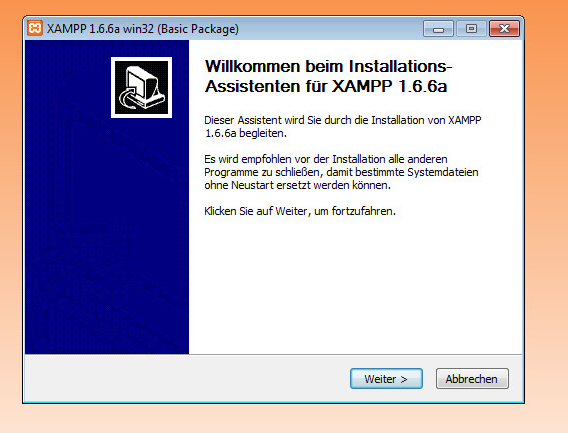
\includegraphics[width=0.7\textwidth]{2_1_1/02.PNG}
        \source{Instellation mit XAMPP Wizard}{Screenshot}{}
    \end{figure}

    \begin{figure}[H]
        \centering
        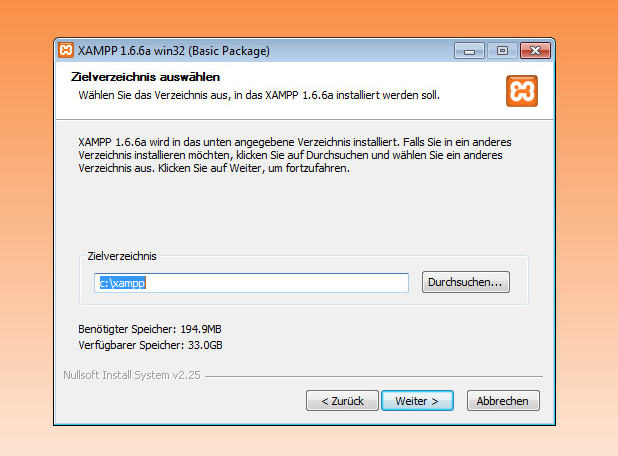
\includegraphics[width=0.7\textwidth]{2_1_1/03.PNG}
        \source{Instellationsverzeichnis}{Screenshot}{}
    \end{figure}

    \begin{figure}[H]
        \centering
        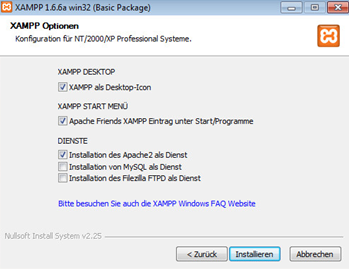
\includegraphics[width=0.7\textwidth]{2_1_1/06_Auswahl.png}
        \source{Konfiguration (Apache)}{Screenshot}{}
    \end{figure}


\subsubsection{Netzwerkfunktionalität beider Workstations}
    \textbf{Planung}
    \begin{itemize}
        \item IPs der WS ermitteln
        \item gegenseitiges pingen der WS
    \end{itemize}

    \begin{figure}[H]
        \centering
        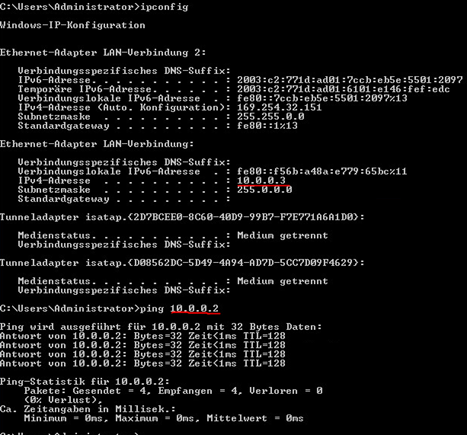
\includegraphics[width=0.7\textwidth]{2_1_2/1.png}
        \source{Ping von Workstation 2 zu Workstation 1}{Screenshot}{}
    \end{figure}

    \begin{figure}[H]
        \centering
        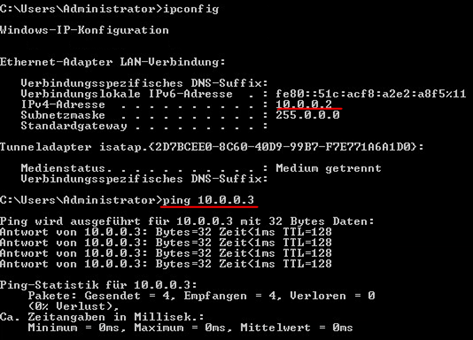
\includegraphics[width=0.7\textwidth]{2_1_2/2.png}
        \source{Ping von Workstation 1 zu Workstation 2}{Screenshot}{}
    \end{figure}


\subsubsection{Netzwerkfunktionalität beider Workstations}
    \textbf{Planung}
    \begin{itemize}
        \item XAMPP installieren 
        \item Apache starten
        \item testen ob Dienst läuft - in browser ip des anderen servers eingeben und prüfen, ob webseite aufgerufen wird 
    \end{itemize}

    \begin{figure}[H]
        \centering
        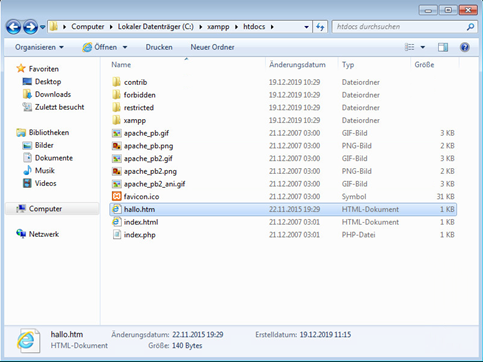
\includegraphics[width=0.7\textwidth]{2_1_3/1.png}
        \source{hallo.htm nach C:{\textbackslash}xampp{\textbackslash}htdocs kopieren}{Screenshot}{}
    \end{figure}

    \begin{figure}[H]
        \centering
        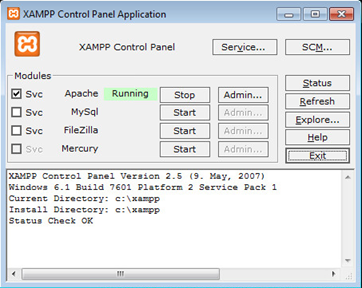
\includegraphics[width=0.7\textwidth]{2_1_3/2.png}
        \source{Apache in XAMPP Starten}{Screenshot}{}
    \end{figure}

    \begin{figure}[H]
        \centering
        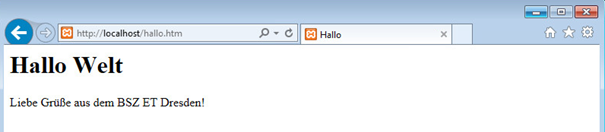
\includegraphics[width=0.7\textwidth]{2_1_3/4.png}
        \source{lokaler Aufruf von hallo.htm}{Screenshot}{}
    \end{figure}

    \begin{figure}[H]
        \centering
        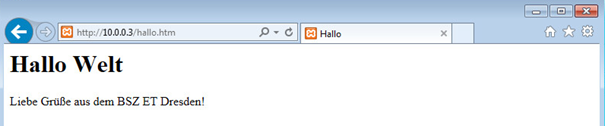
\includegraphics[width=0.7\textwidth]{2_1_3/5.png}
        \source{Aufruf von hallo.htm per IP}{Screenshot}{}
    \end{figure}

\subsubsection{Installieren von Wireshark}
    \begin{figure}[H]
        \centering
        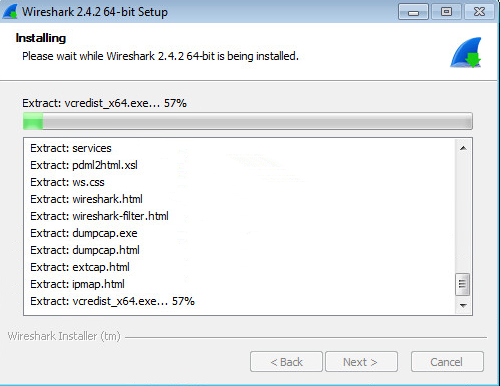
\includegraphics[width=0.7\textwidth]{2_1_4/01.PNG}
        \source{Installation von Wireshark}{Screenshot}{}
    \end{figure}
\pagebreak
\subsection{Aufgaben}
\subsubsection{Aufzeichnung und Analyse der ICMP requests und replys}
    \textbf{Planung}
    \begin{itemize}
        \item Mitschneiden der Pakete und darstellen dieser in Hexadezimalcode
    \end{itemize}
    \begin{figure}[H]
        \centering
        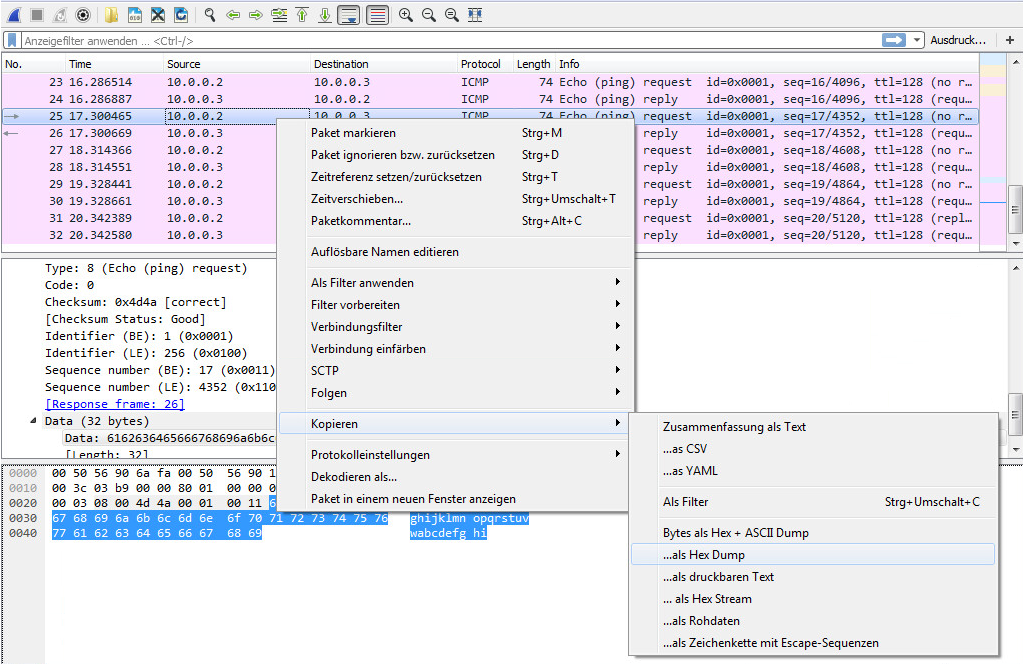
\includegraphics[width=0.7\textwidth]{2_4_1/03-copy.PNG}
        \source{Ausgebenlassen des Dezimalcodes der Pakete}{Screenshot}{}
    \end{figure}

    \subsubsubsection{Fabliches Markieren von Bestandteilen der Paketinhalten}
        \textbf{Request}
        \begin{figure}[H]
            \centering
            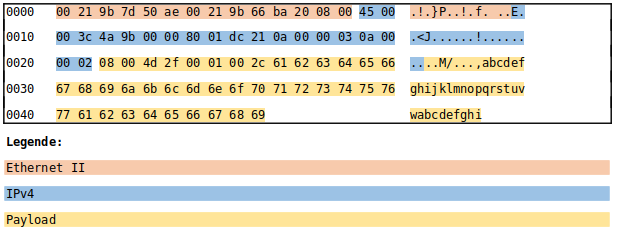
\includegraphics[width=\textwidth]{2_2/a_request.png}
            \source{Wireshark Mitschnitt von ping request}{eigene Zusammenstellung}{}
        \end{figure}
        \pagebreak
        \textbf{Reply}
        \begin{figure}[H]
            \centering
            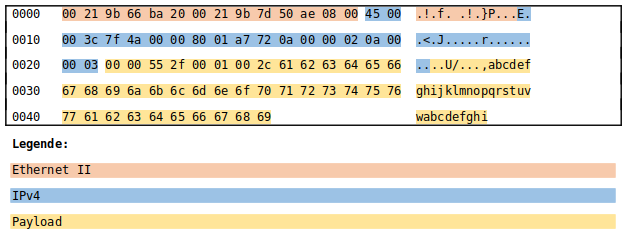
\includegraphics[width=\textwidth]{2_2/a_reply.png}
            \source{Wireshark Mitschnitt von ping reply}{eigene Zusammenstellung}{}
        \end{figure}

    \subsubsubsection{Ermittlung der WS1-IP und des dazugehörigen Hexadezimalcode im IP-Header}
        \textbf{IP Header}
        \begin{figure}[H]
            \centering
            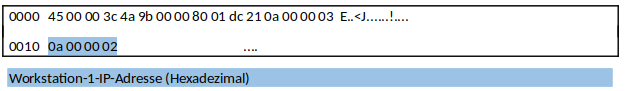
\includegraphics[width=\textwidth]{2_2/b_IP-Header.png}
            \source{IP Header}{eigene Zusammenstellung}{}
        \end{figure}

    \subsubsubsection{Bestimmung der MAC und des NIC}
        \begin{figure}[H]
            \centering
            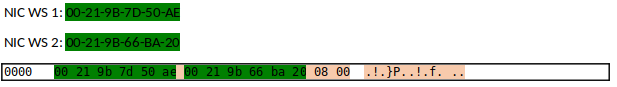
\includegraphics[width=\textwidth]{2_2/c_MAC_NIC.png}
            \source{Wireshark Mitschnitt von ping request}{eigene Zusammenstellung}{}
        \end{figure}
\pagebreak
\subsection{Aufzeichnung der Protokollübertragung von hallo.htm zur WS2}
    \subsubsubsection{Header und Payload jeder Protokollschicht und Zuordnung zu OSI Schichten}
        \textbf{HTTP-Request}
        \begin{figure}[H]
            \centering
            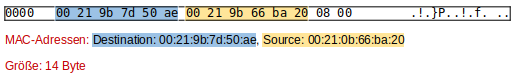
\includegraphics[width=\textwidth]{2_3/1.png}
            \source{Ethernet II (Schicht 2)}{eigene Zusammenstellung}{}
        \end{figure}
        \begin{figure}[H]
            \centering
            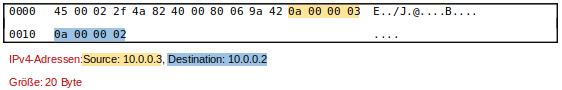
\includegraphics[width=\textwidth]{2_3/2.png}
            \source{IPv4 (Schicht 3)}{eigene Zusammenstellung}{}
        \end{figure}
        \begin{figure}[H]
            \centering
            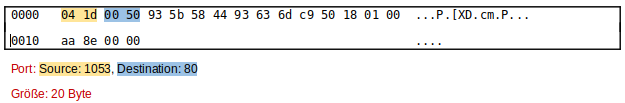
\includegraphics[width=\textwidth]{2_3/3.png}
            \source{TCP (Schicht 4)}{eigene Zusammenstellung}{}
        \end{figure}
        \begin{figure}[H]
            \centering
            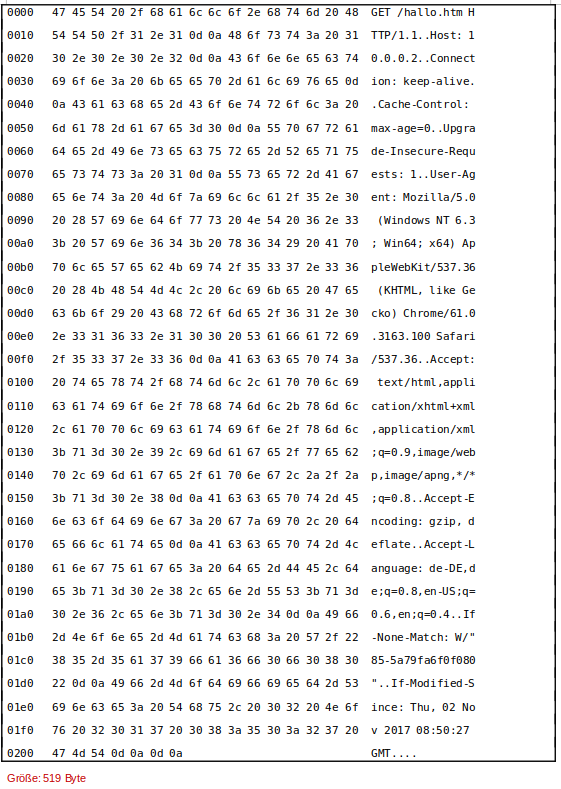
\includegraphics[width=\textwidth]{2_3/4.png}
            \source{HTTP}{eigene Zusammenstellung}{}
        \end{figure}
        \pagebreak
        \textbf{HTTP-Response}
        \begin{figure}[H]
            \centering
            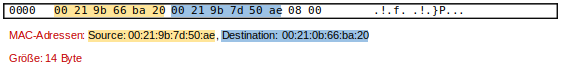
\includegraphics[width=\textwidth]{2_3/5.png}
            \source{Ethernet II (Schicht 2)}{eigene Zusammenstellung}{}
        \end{figure}
        \begin{figure}[H]
            \centering
            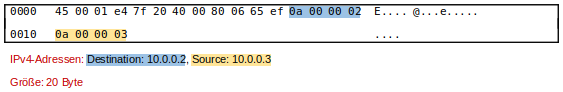
\includegraphics[width=\textwidth]{2_3/6.png}
            \source{IPv4 (Schicht 3)}{eigene Zusammenstellung}{}
        \end{figure}
        \begin{figure}[H]
            \centering
            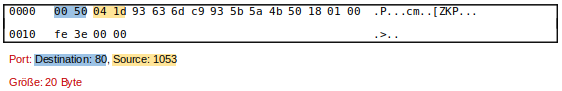
\includegraphics[width=\textwidth]{2_3/7.png}
            \source{TCP (Schicht 4)}{eigene Zusammenstellung}{}
        \end{figure}
        \begin{figure}[H]
            \centering
            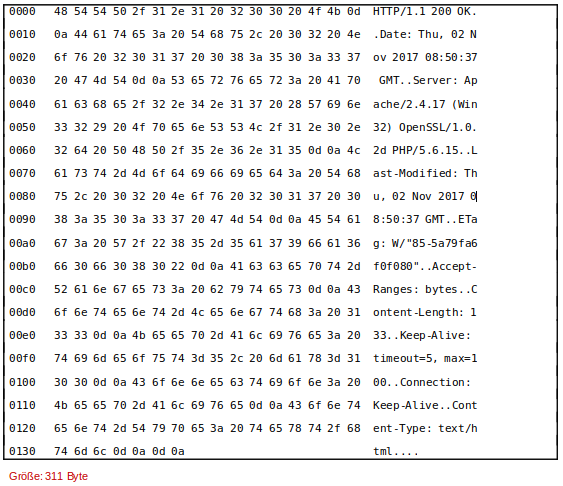
\includegraphics[width=\textwidth]{2_3/8.png}
            \source{HTTP}{eigene Zusammenstellung}{}
        \end{figure}
        \begin{figure}[H]
            \centering
            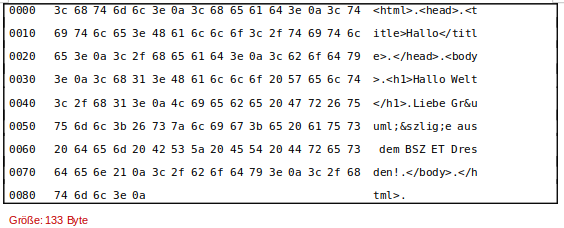
\includegraphics[width=\textwidth]{2_3/9.png}
            \source{Payload}{eigene Zusammenstellung}{}
        \end{figure}

    \subsubsubsection{Verhältnis Payload zur Paketgröße nach DoD-Modell}
        \textbf{Request}
        \begin{longtable}{l|c|l|c}
    \hline
    Schicht & Größe in Byte & Protokoll & \makecell[l]{Verhältnis Payload \\zu Paketgröße}
    \\\hline
    Application & 519 & Data (HTTP) & 90,58 \%
    \\\hline
    Host-to-Host & 20 & Header (TCP) & -
    \\\hline
    Host-To-Host Gesamt & 539 & Data (HTTP + Payload + TCP) & 94,07 \%
    \\\hline
    Internet & 20 & Header (IPv4) & -
    \\\hline
    Internet Gesamt & 559 & Data (HTTP + Payload + TCP + IPv4) & 97,56 \%
    \\\hline
    Network-Access & 14 & Header (Ethernet) & - 
    \\\hline
    Paket Gesamt & 573 & Data (gesamt) & 100 \%

\end{longtable}

        \textbf{Response}
        \begin{longtable}[width=\textwidth]{l|c|l|c}
    \hline
    Schicht & Größe in Byte & Protokoll & \makecell[l]{Verhältnis Payload \\zu Paketgröße}
    \\\hline
    Application & 444 & Data (HTTP + Payload) & 89,14 \%
    \\\hline
    Host-to-Host & 20 & Header (TCP) & -
    \\\hline
    Host-To-Host Gesamt & 464 & Data (HTTP + Payload + TCP) & 93,17 \%
    \\\hline
    Internet & 20 & Header (IPv4) & -
    \\\hline
    Internet Gesamt & 484 & Data (HTTP + Payload + TCP + IPv4) & 97,19 \%
    \\\hline
    Network-Access & 14 & Header (Ethernet) & -
    \\\hline
    Paket Gesamt & 498 & Data (gesamt) & 100 \%
    \\
    \caption{Payload der Response}
\end{longtable}

    \subsubsubsection{Anteil der Nutzdaten zum Frame für den Request und den Response}
        \textbf{Request}\\
        Frame: 573 Bytes \\
        HTML: 0 Bytes\\
        Anteil: 0 \%\\
        \textbf{Response}\\
        Frame: 498 Bytes\\
        HTML: 133 Bytes\\
        Anteil: 26,7 \%

\subsubsection{Umstellung von IPv4 auf IPv6}
    \begin{figure}[H]
        \centering
        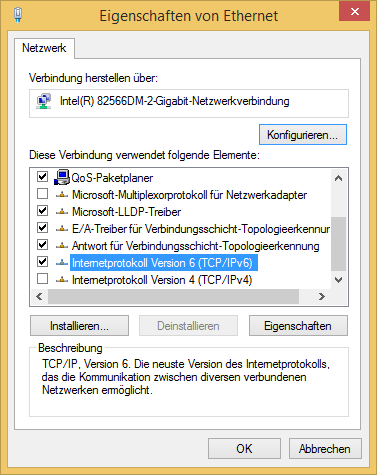
\includegraphics[width=0.5\textwidth]{2_2_3/umstellung_ipv4_ipv6.png}
        \source{Umstellung von IPv4 auf IPv6}{Screenshot}{}
    \end{figure}

    \subsubsubsection{Ausführung des Befehls ipv6 if}

    \begin{figure}[H]
        \centering
        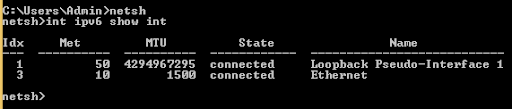
\includegraphics[width=0.5\textwidth]{2_2_3/2.png}
        \source{Ausführung des Befehls ipv6 if}{Screenshot}{}
    \end{figure}

    \subsubsubsection{Testen der Verbindung mit ping, Ermittlung des korrektem Befehls}

    \begin{figure}[H]
        \centering
        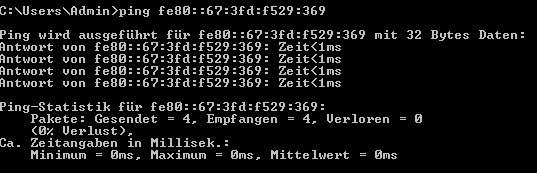
\includegraphics[width=0.5\textwidth]{2_2_3/3.png}
        \source{Ausführen eines Pings auf eine IPv6}{Screenshot}{}
    \end{figure}

    \subsubsubsection{Testen der Aufzeichnung der Kommunikationsbeziehung mit Wireshark und die Unterschiede zu 2.2.1.1}
        \begin{figure}[H]
        \centering
        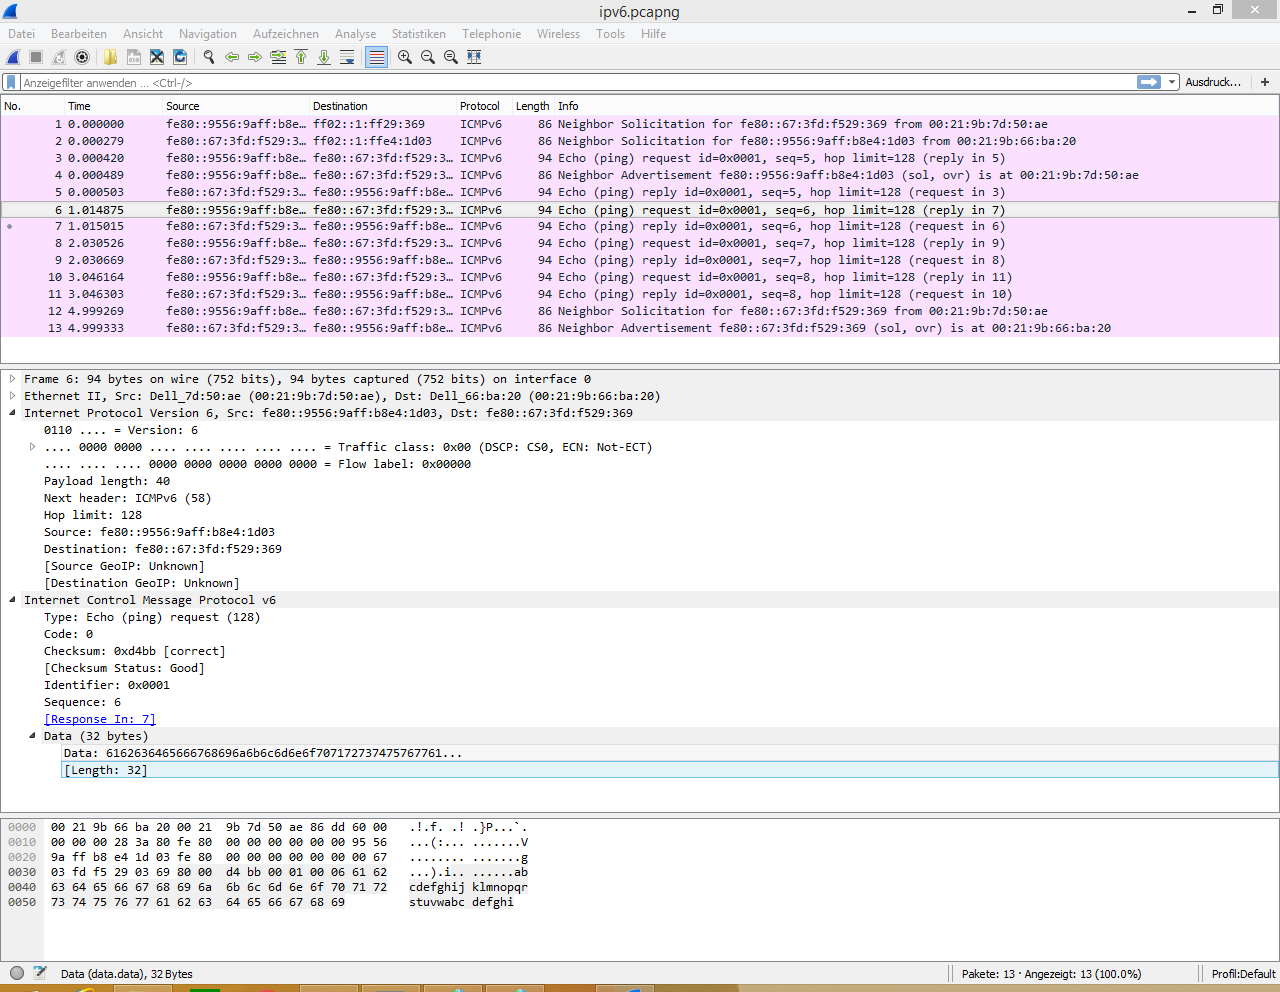
\includegraphics[width=0.5\textwidth]{2_2_3/4.png}
            \source{Mitschnitt via Wireshark request}{Screenshot}{}
        \end{figure}

        \begin{figure}[H]
        \centering
        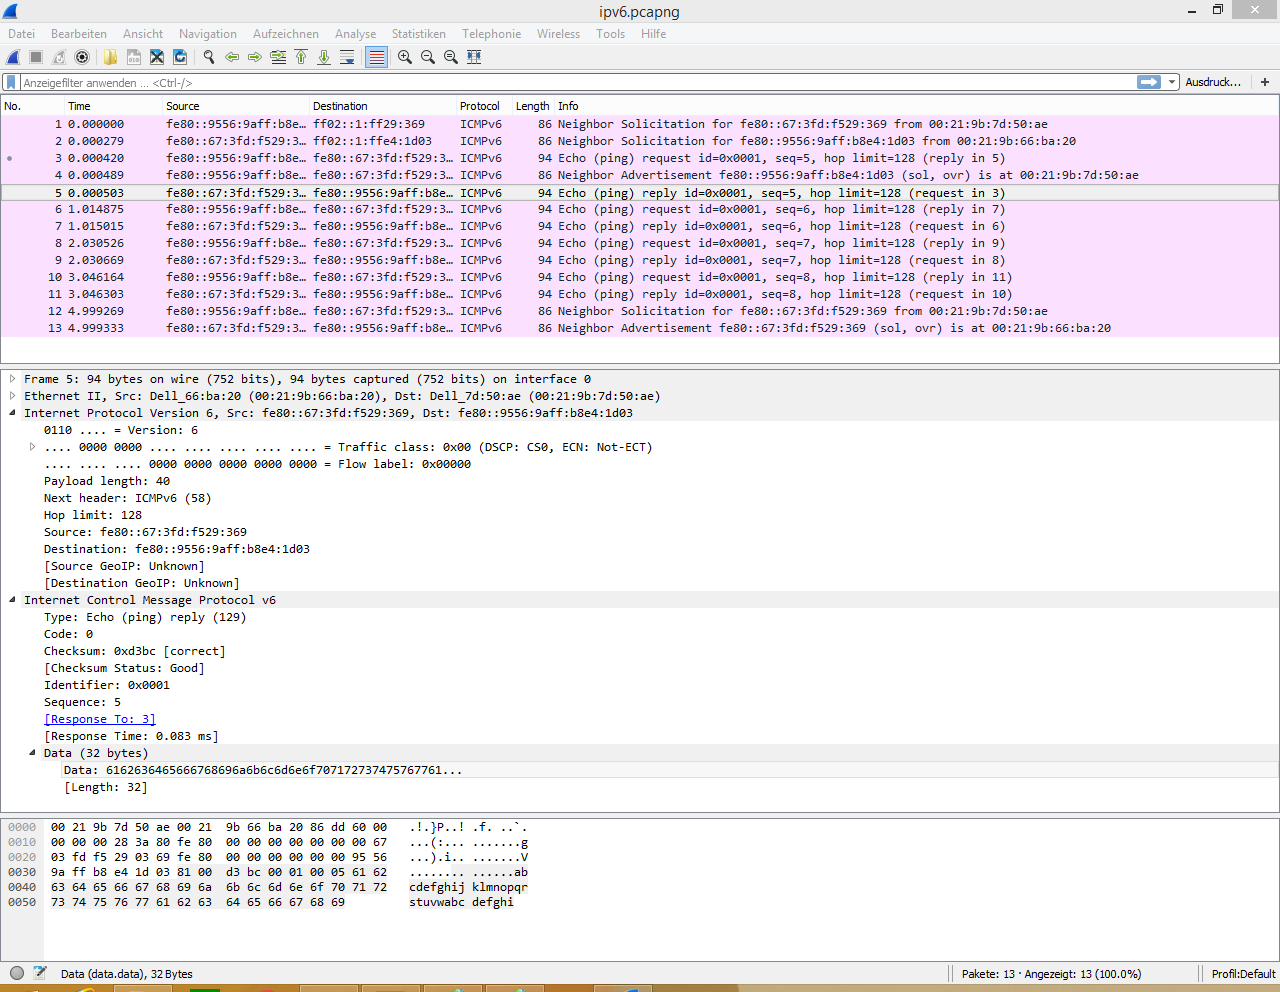
\includegraphics[width=0.5\textwidth]{2_2_3/5.png}
            \source{Mitschnitt via Wireshark reply}{Screenshot}{}
        \end{figure}

        \textbf{Unterschiede zu 2.2.1.1}
        \begin{itemize}
            \item Bei IPv6 ist IP-Header ist größer, da dieser die längeren IPv6 Adressen enthält
            \item Checksum im Payload hat sich verändert
            \item Bei IPv4 gibt es zwei Identifier (BE \& LE), bei IPv6 nur einen
            \item Bei IPv4 gibt es zwei Sequence numbers (BE \& LE), bei IPv6 nur eine sequence (number)
            \item Bei IPv4 gibt es eine “Time to live”, bei IPv6 heißt diese nun “Hop limit”
        \end{itemize}

    \subsubsubsection{Testen einer Ordnerfreigabe zur WS2}
        
        \begin{figure}[H]
        \centering
        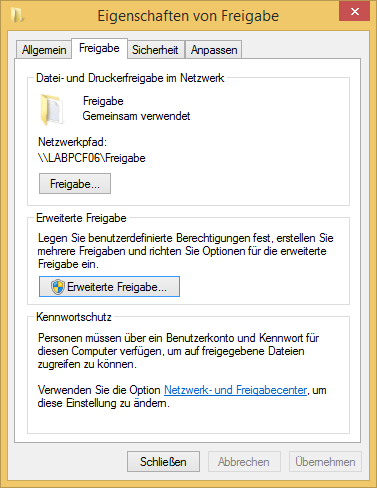
\includegraphics[width=0.5\textwidth]{2_2_3/6.png}
            \source{Eigenschaften der Freigabe}{Screenshot}{}
        \end{figure}

        \begin{figure}[H]
        \centering
        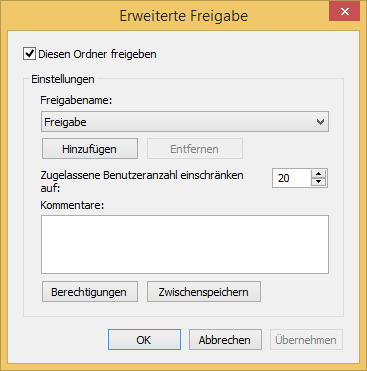
\includegraphics[width=0.5\textwidth]{2_2_3/7.png}
            \source{Erweiterte Freigabe}{Screenshot}{}
        \end{figure}

        \begin{figure}[H]
        \centering
        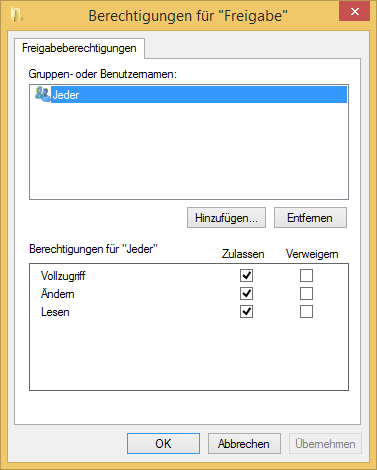
\includegraphics[width=0.5\textwidth]{2_2_3/8.png}
            \source{Berechtigungen für die Freigabe}{Screenshot}{}
        \end{figure}

        \begin{figure}[H]
        \centering
        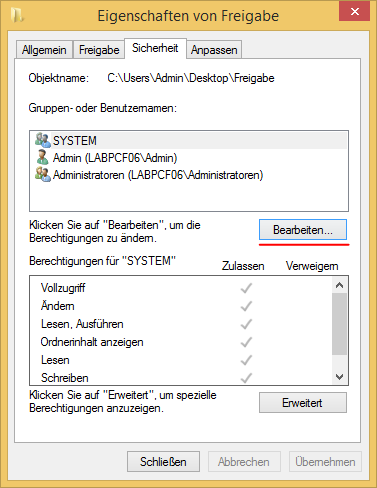
\includegraphics[width=0.5\textwidth]{2_2_3/9.png}
            \source{Bearbeiten der Sicherheit der Freigabe}{Screenshot}{}
        \end{figure}

        \begin{figure}[H]
        \centering
        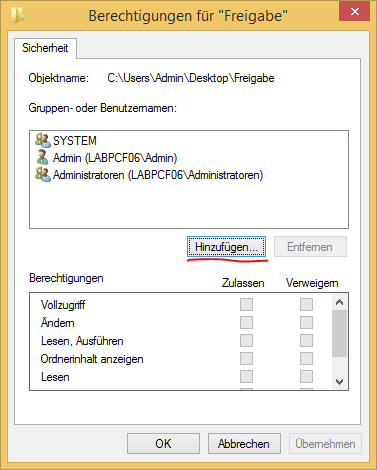
\includegraphics[width=0.5\textwidth]{2_2_3/10.png}
            \source{Berechtigungen hinzufügen}{Screenshot}{}
        \end{figure}

        \begin{figure}[H]
        \centering
        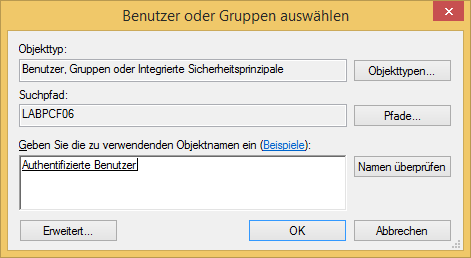
\includegraphics[width=0.5\textwidth]{2_2_3/11.png}
            \source{Einstellen der Bruntzergruppen}{Screenshot}{}
        \end{figure}

        \begin{figure}[H]
        \centering
        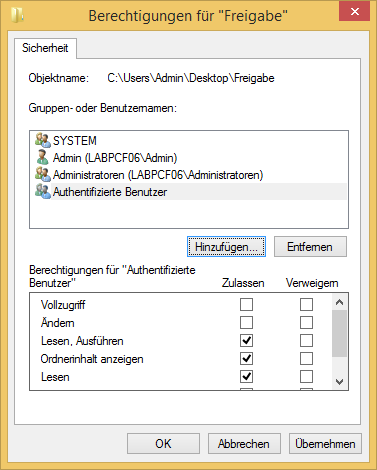
\includegraphics[width=0.5\textwidth]{2_2_3/12.png}
            \source{Berechtigungen für Freigabe}{Screenshot}{}
        \end{figure}

        \begin{figure}[H]
        \centering
        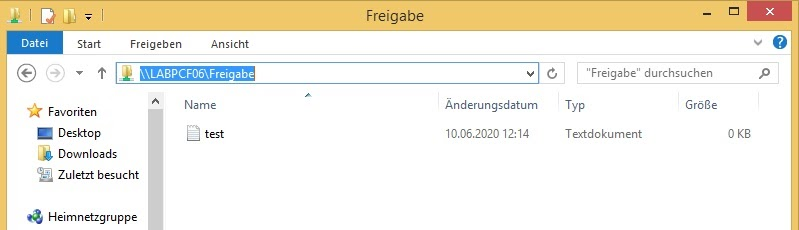
\includegraphics[width=0.5\textwidth]{2_2_3/13.png}
            \source{Anzeige des Freigegebenen Dokuments auf WS1}{Screenshot}{}
        \end{figure}

    \pagebreak
    \section{Abbildungsverzeichnis}
    \listoffigures
    \pagebreak
    \section{Tabellenverzeichnis}
    \listoftables
    \pagebreak
    \section{Quellen}
    \begin{itemize}
    \item https://tools.ietf.org/html/rfc2616\#section-6.2  2.1.2020 13:00 
    \item https://de.wikipedia.org/wiki/IPv6\#Header-Format 2.1.2020 14:45
    \item https://www.lancom-systems.de/docs/LCOS/referenzhandbuch/topics/aa1066622.html 3.1.2020 11:45
    \item https://docs.microsoft.com/en-us/previous-versions/windows/embedded/aa450452(v\%3Dmsdn.10) 3.1.2020 13:00
    \item https://docs.microsoft.com/de-de/previous-versions/windows/embedded/aa450443(v=msdn.10) 3.1.2020 13:00
    \item https://de.wikipedia.org/wiki/Loopback 3.1.2020 13:15
    \item https://de.wikipedia.org/wiki/Time\_to\_Live 3.1.2020 13:30
    \item https://de.wikipedia.org/wiki/OSI-Modell 3.1.2020 14:30
    \item https://www.datenschutzbeauftragter-info.de/osi-modell-so-kommunizieren-rechner/ 6.1.2020 11:00
    \item https://www.black-box.de/de-de/page/26203/Information/Technische-Ressourcen/black-box-erklaert/lan/Layer-2,3-und-4-Switching 6.1.2020 11:00
    \item https://en.wikipedia.org/wiki/Bridging\_(networking) 6.1.2020 14:30
    \item https://www.cpcstech.com/routers-bridges-information.htm 8.1.2020 14:00
    \item https://www.sciencedirect.com/topics/computer-science/gateway-router 8.1.2020 15:00
    \item https://de.m.wikipedia.org/wiki/Metrik\_(Netzwerk) 12.06.2020 10:00
\end{itemize}
    \pagebreak
    \section{Glossar}
    \renewcommand*{\arraystretch}{1.4}
\begin{longtable}{p{0.25\textwidth}p{0.75\textwidth}}
    ICMP & Internet Control Message Protocol - ein Protokoll mit dem überprüft werden kann, ob ein Host im Netzwerk aktiv ist
    \\
    TTL & time to live, gibt beim ICMP die verbleibende maximale Lebenszeit im Netzwerk in Sekunden an
    \\
    MTU & Maximum Transmission Unit, maximale Größe unfragmentierter Datenpakete
    \\
    loopback & Schleifenschaltung mit Nachrichten- oder Informationskanal in dem Sender und Empfänger identisch sind
    \\
    ping & ein Konsolenbefehl, welcher unter fast allen Betriebssystemen funktioniert und ICMP Protokolls Pakete zu interfaces sendet und zurückbekommt, ob diese aktiv sind oder nicht
    \\
    interface &  zu deutsch “Schnittstelle”, hier in dieser Dokumentation wird zumeist mit interface eine virtuelle oder physische Schnittstelle zwischen Netzen gemeint
    \\
    header & Bei Rechnernetzwerken besitzt jedes von einem Rechner versandte Datenpaket einen Header, der Daten über den Absender, Empfänger, Typ und Lebensdauer des Datenpakets enthält.
    \\
    & Beim Hypertext Transfer Protocol (HTTP) werden über den Header HTTP-Cookies und Informationen wie Dateigröße übertragen
    \\
    Payload & Nutzdaten, die keine Steuer- oder Protokollinformationen enthalten. Nutzdaten sind unter anderem Sprache, Text, Zeichen, Bilder und Töne.
    \\
    OSI Schichtmodell & Modell, welches die Ebenen die ein Netzwerk ausmachen beschreibt
    \\
    DoD Schichtmodell & Modell welches Datenübertragungen darstellt
    \\
    link-layer adress & feste Adressen wie die MAC Adresse
\end{longtable}
\end{document}